%\documentclass[a4paper]{scrartcl}
\documentclass[a4paper]{article}
\usepackage{fullpage}
\pagestyle{headings}
\usepackage{mdwlist}
\usepackage{polski}
\usepackage[utf8x]{inputenc}
\usepackage{color}
\usepackage{mathtools}
\usepackage{graphicx}
\usepackage[unicode=true]{hyperref}
\usepackage{multirow}
\usepackage[table]{xcolor}
\usepackage{listings}

\lstset{ %
basicstyle=\footnotesize,       % the size of the fonts that are used for the code
numbers=left,                   % where to put the line\dywiz numbers
numberstyle=\footnotesize,      % the size of the fonts that are used for the line\dywiz numbers
stepnumber=2,                   % the step between two line\dywiz numbers. If it's 1, each line 
% will be numbered
numbersep=5pt,                  % how far the line\dywiz numbers are from the code
frame=single,                   % adds a~frame around the code
}

\begin{document}
\sloppy

\title{coffeecam}
%\subtitle{silniczek graficzny w~coffeescripcie -- wirtualna kamera}
\author{Bartosz Pieńkowski, Barnaba Turek}
\maketitle
\abstract{
Celem serii projektów z~przedmiotu Grafika Komputerowa jest utworzenie prostego silnika graficznego 
(i~zapoznanie się od strony graficznej z~podstawowymi zadaniami grafiki komputerowej, takimi jak rzutowanie,
eliminacja elementów zasłoniętych i~cieniowanie). 

Zdecydowaliśmy się zaimplementować projekt w~języku coffeescript.

Pierwsza część projektu polega na utworzeniu wirtualnej kamery. Kamera ma obsługiwać zmianę pozycji, ogniskowej i~kąta, w~którym jest skierowana.
\section{Wirtualna kamera}
\subsection{Elementy}
Wirtualną kamerę zamierzamy stworzyć korzystając z~następujących elementów:
\begin{enumerate}
  \item Oko
  \item Rzutnia
  \item Scena
\end{enumerate}

Oko i Scena będą dwoma układami współrzędnych.
Rzutnia będzie płaszczyzną zdefiniowaną w układzie współrzędnych oka.

Obiekty, które będziemy renderować będą zdefiniowane w układzie współrzędnych sceny.

Układ współrzędnych oka będzie mógł przemieszczać się w układzie współrzędnych sceny (ruch i obrót kamery).

Zmiana ogniskowej będzie zrealizowana przez przybliżanie i oddalanie rzutni od oka.

\subsection{Działanie kamery}
Działanie kamery będzie polegało na translacji obserwowanych obiektów z układu współrzędnych sceny do układu współrzędnych oka, a następnie rzutowaniu ich na rzutnię 
(zamiana punktów trójwymiarowych na dwuwymiarowe).

Na początku renderowania obrazu zostanie obliczona macierz translacji, służąca do zamiany współrzędnych z układu sceny na układ oka.
Następnie wektory oznaczające wierzchołki brył zostaną przeniesione do układu współrzędnych oka za pomocą wcześniej obliczonej macierzy translacji.
Ostatecznie zostanie wykonane rzutowanie wierzchołków brył na rzutnię, połączenie ich w~czworoboki i~narysowanie ich krawędzi na ekranie.


\subsection{Ruch kamery}
Ruch kamery będzie polegał na obliczeniu nowych współrzędnych oka w~układzie odniesienia oka, a~następnie przetłumaczeniu ich do układu współrzędnych sceny.
Tak obliczone współrzędne zostaną zapisane jako nowe współrzędne kamery.

\subsection{Obrót kamery}
Kamera będzie przechowywać informacje o~swoim obrocie względem układu odniesienia sceny (kąty Eulera).

\section{Plan projektu}
\begin{figure}[h!]
  \caption{Plan projektu}
  \centering
  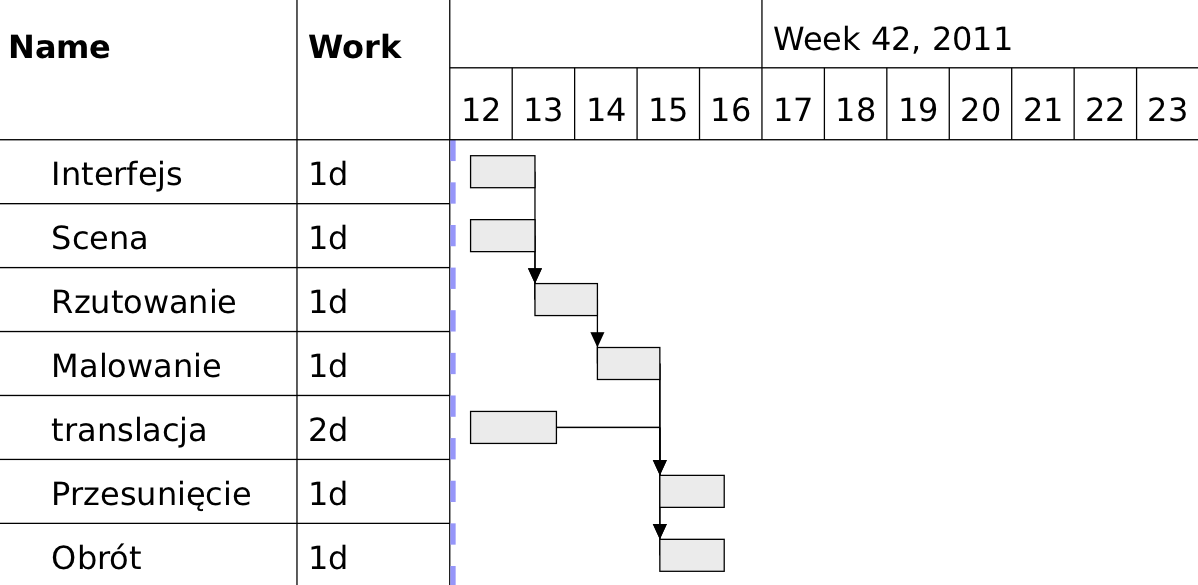
\includegraphics{gantt.png}
\end{figure}


\end{document}
